\subsubsection{Svelte}

\subsubsection*{Správa stavů, předávání vlastností}

Prvním krokem k~vytvoření jednoduchého čítače bude definice komponenty Counter s~reaktivním stavem \emph{count}.

\begin{prog}
// Část souboru Counter.svelte

<script lang="ts">
  let count = 0;
</script>
\end{prog}

Dále vytvoříme komponentu Button z~důvodu dodržování principu DRY a~efektivnějšímu znovupoužití kódu v~budoucnu.
Komponenta bude přijímat vlastnosti \emph{className} a~\emph{onClick}. \emph{ClassName} rozšíří CSS třídy tlačítka a~\emph{onClick} bude obsahovat obslužnou funkci, která se zavolá při kliknutí na tlačítko.
Nyní do šablony přidáme tlačítko a~předáme mu vlastnosti \emph{className} a~\emph{onClick}.
Svelte umožňuje zachytit všechny nedefinované vlastnosti do proměnné \emph{\$\$restProps}. Proměnnou \emph{\$\$restProps} tedy pomocí spread operátoru předáme tlačítku a~tím jej obohatíme o~další vlastnosti. 
Obsah tlačítka, který definujeme mezi párovými značkami Button, vykreslíme pomocí komponenty slot.

\begin{prog}
// Soubor Button.svelte

<script lang="ts">
  export let className: string;
  export let onClick: () => void;
</script>

<!-- Proměnná \$\$restProps obsahuje ostatní vlastnosti, 
  které nejsou v komponentě přijímány pomocí klíčového slova "export". -->
<button
  type="button"
  class="px-4 py-2 rounded-md focus:outline-none \{className\}"
  on:click=\{onClick\}
  \{...\$\$restProps\}
>
  <!-- slot slouží k vykreslení obsahu, 
    který vložíme mezi párové tagy dané komponenty. -->
  <slot />
</button>
\end{prog}

V~Counter komponentě pak v~rámci šablony vykreslíme stav \emph{count} a~Button komponenty, kterým předáme příslušné vlastnosti. 
Pro aktualizaci stavu \emph{count} použijeme obslužné funkce, v~nichž přímo tento stav modifikujeme.

\begin{prog}
// Část souboru Counter.svelte

<script lang="ts">
  import Button from '../components/button/Button.svelte';

  let count = 0;

  const increment = () => (count += 1);
  const decrement = () => (count -= 1);
  const reset = () => (count = 0);
</script>

<div class="bg-gray-200 p-6 rounded-md shadow-md">
  <p class="text-xl font-semibold mb-4">Current count: \{count\}</p>

  <div class="flex gap-4">
    <Button 
      className="bg-blue-500 text-white hover:bg-blue-600" 
      onClick=\{increment\}
    >
      Increment
    </Button>

    <!-- Další komponenty Button... -->
  </div>
</div>
\end{prog}

\subsubsection*{Interakce v uživatelském prostředí}

V~této sekci implementujeme rozbalovací seznam s~možnostmi (dropdown). Tvorbu UI komponenty můžeme začít jak vytvořením HTML struktury, tak definicí funkční stránky komponenty.

My začneme tvorbou šablony, v~níž vytvoříme tlačítko a~seznam možností. 
Otevření možností rozevíracího seznamu zajistíme přidáním \emph{on:click} události na tlačítko a~následně v~obslužné funkci změníme stav \emph{isOpen}.

\begin{prog}
// Část souboru Dropdown.svelte

<div class="rounded-md shadow-sm">
  <!-- Pro poslouchání na události v DOMu můžeme použít syntaxi: 
    on:NÁZEV_UDÁLOSTI=\{OBSLUŽNÁ_METODA\}. -->
  <button
    type="button"
    class=\{`STATICKÉ STYLY... \$\{sizeStyles\} \$\{buttonStyles\}`\}
    on:click|stopPropagation=\{() => (isOpen = !isOpen)\}
  >
    \{selectedOption ? selectedOption.label : placeholder\}
    <!-- Pro podmíněné vykreslovaní můžeme využít bloky
      #if, :else if, :else a /if. -->
    \{#if isOpen\}
      <ArrowUpIcon />
    \{:else\}
      <ArrowDownIcon />
    \{/if\}
  </button>
</div>
\end{prog}

Seznam možností zobrazíme podmíněně na základě \emph{isOpen}. Pro vykreslení možností seznamu (dle vstupu \emph{options}) použijeme blok \emph{\#each}. 
Pro vybrání konkrétní možnosti použijeme \emph{on:click} událost, při které v~anonymní funkci zavoláme funkci \emph{handleOptionClick} s~aktuální položkou ze seznamu.

\begin{prog}
// Část souboru Dropdown.svelte

\{#if isOpen\}
  <div class=\{`STATICKÉ STYLY... \$\{divStyles\}`\}>
    <div 
      class="py-1" role="menu" 
      aria-orientation="vertical" aria-labelledby="options-menu"
    >
      <!-- Pro vykreslení listu (pole hodnot) můžeme využít blok #each. -->
      \{#each options as option\}
        <button
          class=\{`STATICKÉ STYLY... \$\{optionStyles\}`\}
          role="menuitem"
          on:click=\{() => handleOptionClick(option)\}
        >
          \{option.label\}
        </button>
      \{/each\}
    </div>
  </div>
\{/if\}
\end{prog}

Dropdown komponenta bude přijímat vlastnosti \emph{options} a~\emph{onChange}, případně další vlastnosti pro znovupoužitelnost. Pro každou komponentu také vytvoříme jednoznačný identifikátor, který využijeme při uzavírání seznamu.
Obslužná funkce \emph{handleOptionClick} zajistí změnu vybrané možnosti, zavření seznamu a~provede změnu hodnoty v~rodičovské komponentě. 

\begin{prog}
// Část souboru Dropdown.svelte
  
<script lang="ts">
  export let options: ReadonlyArray<Option>;
  export let onChange: (selectedOption: Option | null) => void;
  export let defaultValue: Option | null = null;

  let selectedOption: Option | null = defaultValue;
  let isOpen = false;

  // Toto ID je třeba nastavit na kořenový element dropdown komponenty.
  let dropdownId = `id-\$\{crypto.randomUUID()\}`;

  // Obslužná funkce, která se stará o logiku 
    po kliknutí na jednotlivé položky v dropdownu.
  const handleOptionClick = (option: Option) => \{
    selectedOption = option;
    isOpen = false;
    onChange(option);
  \};
</script>
\end{prog}

K~uzavření jakéhokoli otevřeného seznamu, při kliknutí mimo tento seznam, vytvoříme akci (Svelte action) \emph{clickOutsideDropdown}. 
Uvnitř akce \emph{clickOutsideDropdown} budeme naslouchat na události pointerdown v~DOM. Obslužná funkce pak zajistí spuštění callbacku v~Dropdown komponentě.

\begin{prog}
// Soubor clickOutsideDropdown.ts

export const clickOutsideDropdown = (
  node: HTMLDivElement,
  callback: (event: PointerEvent) => void
) => \{
  const handlePointerDown = (event: PointerEvent) => callback(event);

  document.addEventListener('pointerdown', handlePointerDown);

  return \{
    destroy() \{
      document.removeEventListener('pointerdown', handlePointerDown);
    \},
  \};
\};
\end{prog}

Na kořenový element komponenty přidáme dříve vytvořený unikátní identifikátor a~akci pomocí direktivy \emph{use}. 
Akci následně předáme obslužnou funkci \emph{handleClickOutsideDropdown}, která zavře aktuálně otevřený dropdown.

\begin{prog}
// Část souboru Dropdown.svelte

<script lang="ts">
  // Ostatní stavy, vstupy, funkce v komponentě...

  // Obslužná funkce, která zavře dropdown, pokud uživatel klikne mimo něj.
  const handleClickOutsideDropdown = (\{target\}: PointerEvent) => \{
    if (isOpen && !(target as HTMLElement).closest(`#\$\{dropdownId\}`)) \{
      isOpen = false;
    \}
  \};
</script>
  
<div
  class="relative inline-block text-left"
  id=\{dropdownId\}
  use:clickOutsideDropdown=\{handleClickOutsideDropdown\}
>
  <!-- Vnořené elementy... -->
</div>
\end{prog}

Třídy CSS v~JavaScriptové formě přidáme k~elementu pomocí šablonových literálů a~JS hodnoty.

\subsubsection*{Reaktivita, asynchronní operace}

Uvnitř této sekce se zaměříme na reaktivitu a~asynchronní operace. Naprogramujeme komponentu, která přeloží zadaný text do cílového jazyka. 
Začneme vytvořením komponenty Translator. Komponenta reaktivně (při změně zadaného textu či výstupního jazyka) zavolá API, které vrátí přeložený text. 
V~Translator komponentě využijeme vnořené komponenty, které budou sloužit k~zadání vstupního textu, výběru jazyka a~zobrazení výsledku.

Skrze komponentu LanguageDropdown umožníme uživateli vybrat jazyk, do kterého bude chtít text přeložit. Výstupní jazyk v~rodičovské komponentě změníme přes vlastnost \emph{onChange}.

Pokračujeme implementací komponenty TranslationInput, která umožní zadat vstupní text (\emph{inputText}) přes textové pole. Aktuální hodnotu formulářového prvku nastavíme pomocí \emph{bind:value}. 
V~rodičovské komponentě použijeme \emph{bind}, díky čemuž pak reaktivně aktualizujeme \emph{inputText} v~Translator komponentě.

\begin{prog}
// Část souboru TranslationInput.svelte

<textarea
  bind:value=\{inputText\}
  use:autoresizeTextArea
  class="block w-full min-h-0 p-3 pr-12 pb-8 resize-none !outline-none"
  placeholder="Type to translate ..."
/>

// Část souboru Translator.svelte

<script lang="ts">
  let inputText = '';
</script>

<TranslationInput bind:inputText />
\end{prog}

K~reaktivní změně výšky textového pole použijeme akci \emph{autoresizeTextArea}. Akce přijme element, na kterém se má provést změna výšky. Elementu přidáme listener na událost input. 
V~obslužné funkci následně modifikujeme výšku pole.

\begin{prog}
// Soubor autoresizeTextArea.ts

export const autoresizeTextArea = (element: HTMLTextAreaElement) => \{
  element.addEventListener('input', () => resizeTextArea(element));

  return \{
    destroy() \{
      element.removeEventListener('input', () => resizeTextArea(element));
    \},
  \};
\};

const resizeTextArea = (element: HTMLTextAreaElement) => \{
  // Abychom získali správnou výšku scrollHeight 
    pro textovou oblast, musíme výšku resetovat.
  element.style.height = '0px';
  // Výšku pak nastavíme přímo na nativní prvek.
  element.style.height = `\$\{element.scrollHeight + 36\}px`;
\};
\end{prog}

V rodičovské komponentě budeme odesílat dotazy na Microsoft Translator Text API \cite{translatortextapi} v~momentě, kdy dojde ke změně vstupního textu nebo výstupního jazyka. 
K~tomu využijeme reaktivní prohlášení (reactive statement). V~těle prohlášení nejprve zrušíme předchozí časovač a~pomocí funkce \emph{setTimeout} zavoláme funkci \emph{handleTranslation}. 
Tímto způsobem předejdeme dotazování serveru ihned po změně nějaké vstupní hodnoty. Při zničení komponenty zrušíme časovač a~stávající asynchronní požadavky.

\begin{prog}
// Část souboru Translator.svelte

<script lang="ts">
  // Ostatní stavy, vstupy, funkce v komponentě...
  
  \$: if (inputText.length && outputLanguage) \{
    // Zrušení předchozího časovače.
    clearTimeout(delayTimer);

    // Zpoždění překladu o 300 ms.
    delayTimer = setTimeout(() => handleTranslation(), 300);
  \}

  onDestroy(() => \{
    // Zrušení asynchronního požadavku a časovače při zničení komponenty.
    clearTimeout(delayTimer);
    abortController?.abort();
  \});
</script>
\end{prog}

Účelem asynchronní funkce \emph{handleTranslation} pak je odeslání korektního HTTP POST požadavku na server pomocí fetch API. 
Při úspěšné odpovědi aktualizujeme stav s~přeloženým textem, v~opačném případě nastavíme chybový stav.

Při obdržení odpovědí ze serveru vykreslíme přeložený text uživateli pomocí komponenty TranslationOutput. 
Komponentě předáme výstupní text spolu s~dalšími vlastnostmi, na základě kterých v~šabloně podmíněně vykreslíme přeložený text, chybu nebo načítání.

\subsubsection*{Tvorba formulářů, validace}

Svelte, stejně jako React, nepodporuje pokročilou správu formulářů. Můžeme však využít knihovny třetích stran, jako např.~svelte-forms-lib nebo Superforms, které nám umožní lépe spravovat a~validovat formuláře. 
V~této sekci vytvoříme komponentu pro jednoduchou investiční kalkulaci s~využitím knihovny \emph{svelte-forms-lib} \cite{svelteformslib}. 
Komponenta InvestForm bude obsahovat formulář pro zadání vstupních hodnot a~komponentu FutureValuesInfo pro zobrazení výsledků kalkulace.

Začneme implementací reaktivního formuláře, který bude přijímat počáteční hodnoty (\emph{defaultValues}) a~\emph{investFormData} k~předávání hodnot formuláře do rodičovské komponenty. 
Strukturu formuláře popíšeme v~typu \emph{InvestFormData}. Pomocí funkce \emph{createForm} z~knihovny \emph{svelte-forms-lib} vytvoříme instanci formuláře, které předáme \emph{defaultValues} do vlastnosti \emph{initialValues}. 
V~rámci nastavení formuláře také definujeme validační schéma pomocí knihovny \emph{yup} \cite{yuplibrary} a~\emph{onSubmit} obslužnou funkci. 
Knihovnu yup volíme, jelikož je jedinou kompatibilní možností s~knihovnou \emph{svelte-forms-lib} ve verzi 2.0.1. 
% vlastnost validationSchema musí být typu ObjectSchema<any>, který je definován jen a pouze v knihovně yup:
% import type {ObjectSchema} from 'yup';
% validationSchema?: ObjectSchema<any>;

\begin{prog}
// Část souboru InvestForm.svelte

<script lang="ts">
  const validationSchema = object().shape(\{
    oneOffInvestment: number().min(20).max(99_999_999).required(),
    investmentLength: number().min(3).max(60).required(),
    averageSavingsInterest: number().min(0).max(10).required(),
    averageSP500Interest: number().required(),
  \});
</script>
\end{prog}

Aby nastavená výstupní data (\emph{investFormData}) odpovídala typu \emph{InvestFormData}, musíme transformovat hodnoty formuláře pomocí funkce \emph{cast} na validačním schématu. V~opačném případě budou hodnoty typu string. 
Z~\emph{createForm} následně získáme obslužné funkce \emph{handleChange} a~\emph{handleSubmit}, dále stavy formuláře \emph{form}, \emph{errors} a~\emph{isValid}. Ke stavům formuláře přistupujeme pomocí \$, protože jde o~stores observables.

\begin{prog}
// Část souboru InvestForm.svelte

<script lang="ts">
  const \{form, errors, isValid, handleChange, handleSubmit\} = createForm(\{
    initialValues: defaultValues,
    validationSchema,
    onSubmit: values => \{
      // Převede hodnoty formuláře na typ InvestFormData.
      investFormData = validationSchema.cast(values);
    \},
  \});
</script>
\end{prog}

Do šablony přidáme form s~\emph{on:submit} událostí, které předáme \emph{handleSubmit}. Pokračujeme vytvořením formulářových prvků. 
Jednotlivé prvky propojíme s~reaktivním formulářem pomocí \emph{bind:value} a~události \emph{on:change}, do které přiřadíme funkci \emph{handleChange}. 
Chyby formuláře získáme z~\emph{errors} a~vykreslíme je pod formulářovými prvky. 
Také přidáme tlačítko s~typem submit, které se postará o~odeslání formuláře a~zavolání obslužné funkce \emph{onSubmit}.

\begin{prog}
// Část souboru InvestForm.svelte

<form on:submit=\{handleSubmit\}>
  <div class="md:flex md:gap-4">
    <div class="mb-4 md:w-1/2">
      <InputLabel id="oneOffInvestment">
        One-off investment (20-99.999.999€)
      </InputLabel>

      <!-- Propojení formulářového prvku se stavem formuláře
        pomocí bind:value=\{\$form.NÁZEV_POLE\}. -->
      <!-- Propagace změn do stavu formuláře 
        zajišťuje on:change=\{handleChange\}. -->
      <input
        id="oneOffInvestment"
        type="number"
        on:change=\{handleChange\}
        bind:value=\{\$form.oneOffInvestment\}
        class="STATICKÉ STYLY..."
      />

      \{#if \$errors.oneOffInvestment\}
        <p class="text-red-500 text-xs italic mt-1">
          Please enter a valid amount of one-off investment (positive number).
        </p>
      \{/if\}
    </div>
  </div>

  <!-- Další formulářové prvky... -->

  <button
    type="submit"
    disabled=\{!\$isValid\}
    class="STATICKÉ STYLY..."
  >
    Calculate
  </button>
</form>
\end{prog}

Pokračujeme tím, že v~rodičovské komponentě pomocí \emph{bind} získáme aktuální hodnoty formuláře (\emph{investFormData}). Po změně hodnot formuláře hodnoty transformujeme pomocí funkce \emph{futureValuesCalculator}. 
Výsledek (\emph{futureValues}) pak zobrazíme v~komponentě FutureValuesInfo. Jednotlivé výsledky budou zobrazeny ve vnořených komponentách FutureValueInfo. 
K~modifikaci vstupní hodnoty v~komponentě FutureValueInfo použijeme reactive statement.

\begin{prog}
// Soubor FutureValueInfo.svelte
  
<script lang="ts">
  export let futureValue: number;

  \$: localizedFutureValue = `\$\{futureValue.toLocaleString('de-DE')\}€`;
</script>

<div class="p-1 sm:w-1/2">
  <p class="text-xl font-semibold mb-2 text-gray-800"><slot /></p>
  <p class="text-5xl font-bold">\{localizedFutureValue\}</p>
</div>
\end{prog}

\subsubsection*{Modularita, použití knihoven}

Nyní vytvoříme webovou hru, ve které bude úkolem uživatele uhádnout název státu na základě poskytnutých nápověd. Práci si zlehčíme využitím externích knihoven. 
Během hry se postupně odkryje 8 nápověd, které uživateli pomohou uhádnout název daného státu. Mezi klíčovými prvky bude textové pole pro zadání názvu země a~potvrzovací tlačítko. 
Součástí hry bude také seznam zemí, které uživatel hádal a~modální okna pro vyhodnocení hry.

Začneme implementací rodičovské komponenty, jejíž úkolem bude získat země z~REST Countries API \cite{restcountriesapi}. 
K~tomu využijeme balíčky \emph{axios} \cite{axioslib} a~\emph{@tanstack/svelte-query} \cite{tanstackquerylib}. 
Knihovna \emph{@tanstack/svelte-query} umožní snadnou správu asynchronních operací. Její API poskytuje např.~podporu načítacích i~chybových stavů, také rušení či opakování dotazů a~mnoho dalších funkcí. 
Nejdříve inicializujeme \emph{svelte-query} klienta v~rámci poskytovatele \emph{QueryClientProvider} v~\emph{App.svelte}.

\begin{prog}
// Část souboru App.svelte

<script lang="ts">
  // Importy, konstanty, funkce...  

  // Vytvoření instance QueryClient pro HTTP dotazy.
  const queryClient = new QueryClient();
</script>

<QueryClientProvider client=\{queryClient\}>
  <!-- Layout aplikace... -->
</QueryClientProvider>
\end{prog}

Dále vytvoříme funkci \emph{useAllCountries}, která vrátí výsledek HTTP dotazu (\emph{CreateQueryResult}) pomocí funkce \emph{createQuery}. 
Argumentem funkce \emph{createQuery} bude objekt s~názvem dotazu (\emph{queryKey}) a~funkce, která vykoná dotaz (\emph{queryFn}).

\begin{prog}
// Část souboru queries.ts

export const useAllCountries = (): CreateQueryResult<Countries, Error> => \{
  return createQuery<Countries>(\{
    queryKey: ['allCountriesQuery'], queryFn: getAllCountries
  \});
\};
\end{prog}

Dotaz na server provede asynchronní funkce \emph{getAllCountries}, v~níž využijeme převzatou asynchronní funkci \emph{requestHandler} \cite{axiosrequesthandler} a~knihovnu \emph{axios} \cite{axioslib}. 
Po získání odpovědi ošetříme chyby a~vrátíme výsledek.

\begin{prog}
// Část souboru getAllCountries.ts

export const getAllCountries = async () => \{
  const fetchCountriesData = requestHandler<object, Countries>(() =>
    axios.request(getRequestConfig())
  );
  const response = await fetchCountriesData(\{\});

  if (response.code === 'error') \{
    throw new Error(
      `There was an error with getting the countries data 
      (\$\{response.error.message\}). Please reload the page.`
    );
  \}

  if (response.data.length === 0) \{
    throw new Error('There are no countries to guess. Please try again later.');
  \}

  return getSortedCountriesByName(response.data);
\};
\end{prog}

V~rámci rodičovské komponenty dostaneme výsledek dotazu a~uložíme jej do proměnné \emph{countries}. Pomocí vlastností \emph{isError} a~\emph{data} podmíněně vykreslíme jednotlivé komponenty. 
V~případě chyby zobrazíme komponentu ErrorAlert. Když úspěšně získáme pole zemí, vykreslíme komponentu CountryGuesser. LoadingSkeleton zobrazíme, pokud se nezobrazí žádná z~předchozích komponent.

\begin{prog}
// Soubor CountryGuesserWrapper.svelte

<script lang="ts">
  // Importy...

  const countries = useAllCountries();
</script>

\{#if \$countries.isError\}
  <div 
    class="container flex flex-col justify-center justify-items-center mx-auto"
  >
    <ErrorAlert message=\{\$countries.error.message\} />
  </div>
\{:else if \$countries.data\}
  <CountryGuesser countries=\{\$countries.data\} />
\{:else\}
  <div 
    class="container flex flex-col justify-center justify-items-center mx-auto"
  >
    <LoadingSkeleton />
  </div>
\{/if\}
\end{prog}

Komponenta CountryGuesser zobrazí jednotlivé herní prvky a~bude vyhodnocovat průběh hry. 
Začneme definicí stavů a~náhodně vybereme náhodnou zemi (\emph{randomCountry}), kterou uživatel bude hádat. 
V~hooku \emph{onMount} zavoláme funkci \emph{polyfillCountryFlagEmojis}. Při namontování komponenty tak zajistíme zobrazení ikon vlajek v~prohlížečích, které to přímo nepodporují. 
Prohlížeč uživatele však musí podporovat emojis a~webové fonty. Funkce \emph{polyfillCountryFlagEmojis} přidá do hlavičky stránky webový font Twemoji Country Flags. 
Aby se font použil, přidáme jej do CSS stylů.

\begin{prog}
// Část souboru app.css

@layer base \{
  html \{
    font-family: 'Twemoji Country Flags', 'ALTERNATIVNÍ_FONTY...';
  \}
\}
\end{prog}

Poté naprogramujeme obslužné funkce \emph{handleEvaluateGuessAndUpdateState}, \emph{handleSetInitialState}, které budou sloužit k~aktualizaci stavu hry. 
V~šabloně zobrazíme jednotlivé herní prvky a~modální okna při výhře či prohře.

Pomocí HintBoxes komponenty postupně zobrazíme nápovědy. Dle vstupu \emph{randomCountry} budeme reaktivně vytvářet pole nápověd, jelikož \emph{randomCountry} se může změnit. 
V~šabloně posléze vykreslíme napovědy pomocí HintBox komponent. HintBox dynamicky vykreslí název a~SVG ikonu nápovědy, textovou nápovědu, případně obrázek vlajky státu.

\begin{figure}[htb]
	\centering
		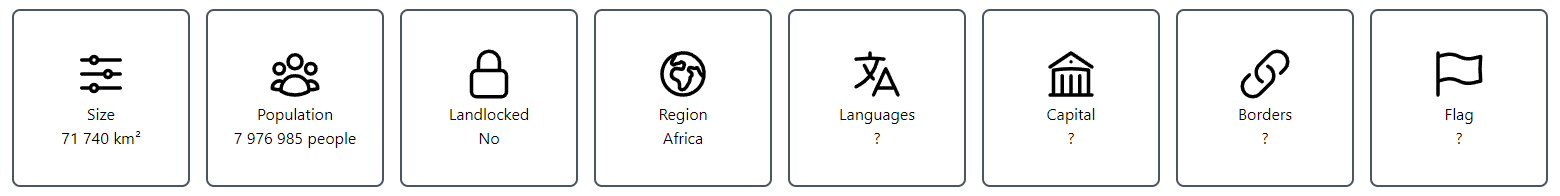
\includegraphics[width=.97\textwidth]{images/HintBoxes.jpg}
	\caption[HintBoxes]{HintBoxes - vlastní zpracování}
	\label{fig:sveltehintboxes}
\end{figure}

Komponenta \emph{CountryGuessInput.svelte} umožní uživateli zadání názvu země (uživatelova tipu). Začneme šablonou, kde vytvoříme formulářový prvek pro zadání tipu a~potvrzovací tlačítko. 
Dále také podmenu textového pole, které zobrazí nejpodobnější země na základě zadaného textu (filtrované země). Přidáme obslužné funkce pro akce a~události nad formulářem, které následně doimplementujeme.

\begin{figure}[htb]
	\centering
		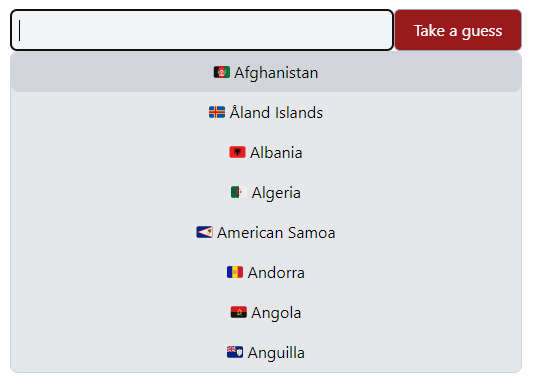
\includegraphics[width=.5\textwidth]{images/CountryGuessInput.jpg}
	\caption[CountryGuessInput]{CountryGuessInput - vlastní zpracování}
	\label{fig:sveltecountryguessinput}
\end{figure}

Ve skriptové části, na základě vstupu \emph{countries}, získáme pole všech zemí bez těch, které uživatel již hádal (\emph{countriesWithoutAlreadyGuessed}). 
Následně definujeme a~inicializujeme ostatní stavy komponenty. Po kliknutí na potvrzovací tlačítko zavoláme funkci \emph{handleGuessButtonClick}. 
V~tělě funkce zavoláme obslužnou funkci \emph{evaluateGuessAndUpdateState}, pomocí níž vyhodnotíme stav hry v~rodičovské komponentě. 
Dále také funkci \emph{handleChangeSelectedGuess}, která aktualizuje aktuální tip, filtrované země a~uzavře podmenu. 
Funkce \emph{handleInputChange} převede tip uživatele do daného formátu, aktualizuje aktuální tip a~filtrované země. Ovládání textového pole pomocí klávesnice umožní funkce \emph{handleKeyDown}.

V~pomocné funkci \emph{updateGuessAndFilteredCountries} nejprve získáme filtrované země podle uživatelova tipu. Pak aktualizujeme stavy \emph{currentGuess}, \emph{isValidGuess} a~\emph{filteredCountries}. 
Funkce \emph{clampSelectedGuessIndex} zajistí, aby index vybrané země byl v~požadovaném rozmezí (0 až počet filtrovaných zemí). 
K~modifikaci stavu \emph{selectedGuessIndex} použijeme funkci \emph{changeSelectedGuessIndex}, která index aktualizuje o~hodnotu předanou v~argumentu. 
Tip uživatele pomocí funkce \emph{convertToFormattedGuess} převedeme tak, aby začínal velkým písmenem a~zbytek řetezce byl složen z~malých písmen.

Pro zobrazení všech již hádaných zemí uživatelem vytvoříme komponentu GuessedCountriesList. 
Ze vstupních vlastností \emph{countries}, \emph{guessedCountries} a~\emph{randomCountry} získáme proměnnou \emph{enrichedGuessedCountries}. 
Jde o~uživatelem hádané země s~vlajkou a~vzdáleností od \emph{randomCountry}. K~převodu využijeme JS funkci z~jiného souboru. 
Vzdálenost zemí vypočteme pomocí knihovny \emph{calculate-distance-between-coordinates} \cite{distancebetweencoordinates}, která exportuje funkci \emph{getDistanceBetweenTwoPoints}. 
Proměnnou \emph{enrichedGuessedCountries} poté vykreslíme v~šabloně.

\begin{figure}[htb]
	\centering
		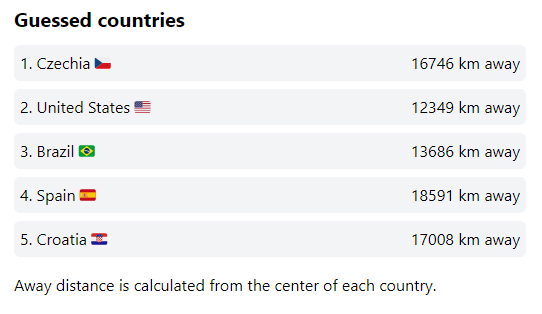
\includegraphics[width=.7\textwidth]{images/GuessedCountriesList.jpg}
	\caption[GuessedCountriesList]{GuessedCountriesList - vlastní zpracování}
	\label{fig:svelteguessedcountrieslist}
\end{figure}

Závěrem vytvoříme modální okna, která vykreslíme při výhře nebo prohře. Stavy \emph{isWinModalOpen} a~\emph{isLoseModalOpen} aktualizujeme uvnitř funkce \emph{handleEvaluateGuessAndUpdateState} v~CountryGuesser. 
Na základě těchto stavů podmíněně zobrazíme daná modální okna. Oběma oknům předáme \emph{randomCountry} a~obslužnou funkci \emph{handleClose}. Do výherního modálu také počet potřebných pokusů. 
V~jednotlivých komponentách (WinModal, LoseModal) vykreslíme komponentu BaseModal, která bude sloužit jako šablona pro obě okna. Do této komponenty pak předáme titulek, obsah modálu a~obslužnou metodu \emph{handleClose}. 
V~šabloně BaseModal vykreslíme základní strukturu modálního okna s~dynamickými vlastnostmi.

\subsubsection*{Routování a layout aplikace}

Aplikaci rozdělíme do tří částí: hlavičky, patičky a~samotného obsahu, v~němž vykreslíme jednotlivé komponenty. Uživatel se bude moci přepínat mezi jednotlivými stránkami přes navigační menu. 

Pro routování v~aplikaci využijeme knihovnu \emph{svelte-spa-router} \cite{sveltesparouterlib}. Nejprve vytvoříme seznam cest aplikace (\emph{appRoutes}).

\begin{prog}
// Část souboru appRoutes.ts

interface AppRoute \{
  name?: string;
  path: string;
  component: ComponentType;
\}

export const appRoutes: ReadonlyArray<AppRoute> = [
  \{
    name: 'Home',
    path: '/',
    component: Landing,
  \},
  \{
    name: 'Counter',
    path: '/counter',
    component: Counter,
  \},
  // Další cesty...
  \{
    path: '*',
    component: PageNotFound,
  \},
];
\end{prog}

Uvnitř hlavní komponenty transformujeme \emph{appRoutes} do požadovaného formátu (typu \emph{RouteDefinition}) a~výsledek uložíme do proměnné \emph{routes}. 
V~šabloně zobrazíme hlavičku, patičku a~\emph{Router}, kterému předáme proměnnou \emph{routes}. 
\emph{Router} následně vykreslí šablonu na základě aktuální URL adresy.

\begin{prog}
// Část souboru App.svelte

<script lang="ts">
  // Importy...

  // Vytvoření cest pro svelte-spa-router.
  const routes: RouteDefinition = appRoutes.reduce(
    (routesMap, route) => routesMap.set(route.path, wrap(\{
      component: route.component
    \})),
    new Map()
  );
</script>

<QueryClientProvider client=\{queryClient\}>
  <div class="min-h-screen flex flex-col">
    <Header />

    <main class="flex-grow p-8">
      <!-- Router vykresluje šablonu (komponentu) pro aktuální URL adresu. -->
      <Router \{routes\} />
    </main>

    <Footer />
  </div>
</QueryClientProvider>
\end{prog}

Hlavička zobrazí odkazy na jednotlivé stránky. Architekturu a~vzhled navigačního menu převezmeme např.~od Flowbite. 
V~rámci komponenty Header vypíšeme cesty aplikace pomocí HTML elementu a, na nějž přidáme atribut href. 
Dále přidáme také akce \emph{link} a~\emph{active}, které poskytuje \emph{svelte-spa-router}. 
Akci \emph{active} předáme objekt, kde přes vlastnosti \emph{className} a~\emph{inactiveClassName} nastavíme požadovanou CSS třídu podle toho, zda je odkaz aktivní nebo neaktivní. 
K~nastavení aria-current použijeme \emph{location} objekt ze \emph{svelte-spa-router}, díky kterému získáme aktuální URL.

\begin{prog}
// Část souboru Header.svelte

\{#each routes as route\}
  <li>
    <!-- svelte-spa-router poskytuje akce "link" a také "active". -->
    <!-- Akce active slouží k nastavení CSS na základě aktivního odkazu. -->
    <a
      href=\{route.path\}
      class="block py-2 pr-4 pl-3 lg:p-0"
      use:link
      use:active=\{\{
        className: 'STATICKÉ STYLY PRO AKTIVNÍ ODKAZ...',
        inactiveClassName: 'STATICKÉ STYLY PRO NEAKTIVNÍ ODKAZ...',
      \}\}
      aria-current=\{route.path === \$location ? 'page' : null\}
    >
      \{route.name\}
    </a>
  </li>
\{/each\}
\end{prog}

Stavy \emph{isMobileNavOpen} a~\emph{isDarkMode} umožní ovládat zobrazení mobilní navigace a~barevného režimu. K~uložení preference tmavého režimu využijeme LocalStorage v~prohlížeči. 
Logiku pro přepnutí barevného režimu zavoláme v~hooku \emph{beforeUpdate}. Tento hook se spustí po změně lokálního stavu, ale před aktualizací HTML.

\begin{prog}
// Část souboru Header.svelte

beforeUpdate(() => \{
  if (isDarkMode) \{
    document.documentElement.setAttribute('data-mode', 'dark');
    localStorage.setItem('data-mode', 'dark');
  \} else \{
    document.documentElement.removeAttribute('data-mode');
    localStorage.removeItem('data-mode');
  \}
\});
\end{prog}